
\chapter{Report of the U.S. CMS Resource Manager}

The funding provided by DOE and NSF to the U.S.\ CMS Operations Program
for 2002 through 2015, as well as the funding guidance for 2016 through 2019,
is shown in Figure~\ref{fig:funding_profile}.

\begin{figure}[hbtp]
  \begin{center}
    \resizebox{6.25in}{!}{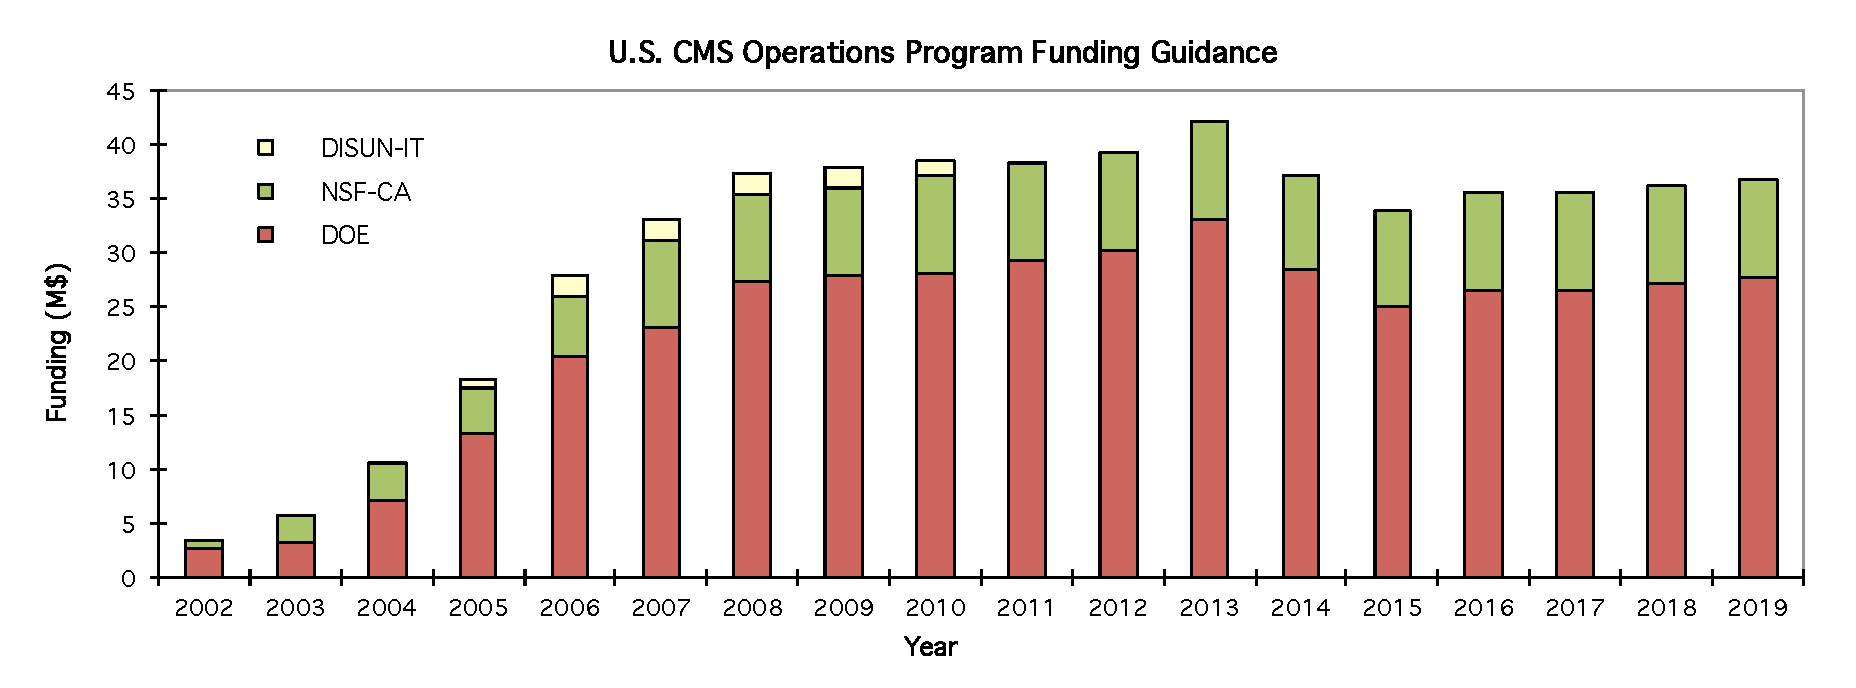
\includegraphics{figures/CY15_Funding_Profile.pdf}}
    \caption{The annual U.S.\ CMS Operations Program funding provided by
DOE and NSF.  For 2002 through 2015 the chart shows the actual funding,
while for 2016 onward the current funding guidance is shown.}
    \label{fig:funding_profile}
  \end{center}
\end{figure}

Resources are distributed and tracked across the three areas through
which the Operations Program is implemented:  Detector Operations (DetOps),
Software and Computing (S\&C), and Common Operations (ComOps).
ComOps is a category for items that would otherwise belong in both, or
neither, of the other two categories.

Internal budget reviews for calendar year 2015 took place in August and
September of 2014.  Through this process, U.S.\ CMS Management
developed a detailed spending plan.  This plan was further refined
through the March 2015 joint NSF/DOE Operations Program review.

Primarily during the first quarter of the calendar year,
Statement of Work (SOW) agreements were established with each institution
that is providing a deliverable in exchange for Operations Program funding.
The SOWs specify the tasks to be carried out, as well as any portions of
salaries, materials and services (M\&S), travel funding, or cost of living
adjustments (COLA) to be paid from the Operations Program budget.
The SOWs must be approved by U.S.\ CMS Operations Program management,
by the Fermilab Director Designee, and by
representatives of the collaborating group and institution.
Through September of 2015, a total of 109 SOWs (71 DOE and 38 NSF) were produced
and approved.  After a SOW is approved, any additional changes are considered and,
if approved, enacted through a Change Request procedure.

Table~\ref{tab:change_log} shows the Spending Plan Change Log which
captures revisions that were made prior to SOW approvals, as well as
modifications implemented through Change Requests.  The information is
reported here down to the level-2 subsystem categories within DetOps, S\&C,
and ComOps.  There was a relatively large number of Change Requests
relating to Phase 2 (HL-LHC) Upgrade R\&D this quarter.  These are
summarized separately in Table~\ref{tab:phase2_change_log}.
The CY15 spending plan, as of the end of Q3, is shown for DOE
and NSF funds in Table~\ref{tab:spending_plan}.  The plan will
continue to evolve slightly as Change Requests are executed.

\begin{table}[hbtp]
  \begin{center}
    \caption{Spending Plan Change Log for CY15 Q3}
    \resizebox{6.25in}{!}{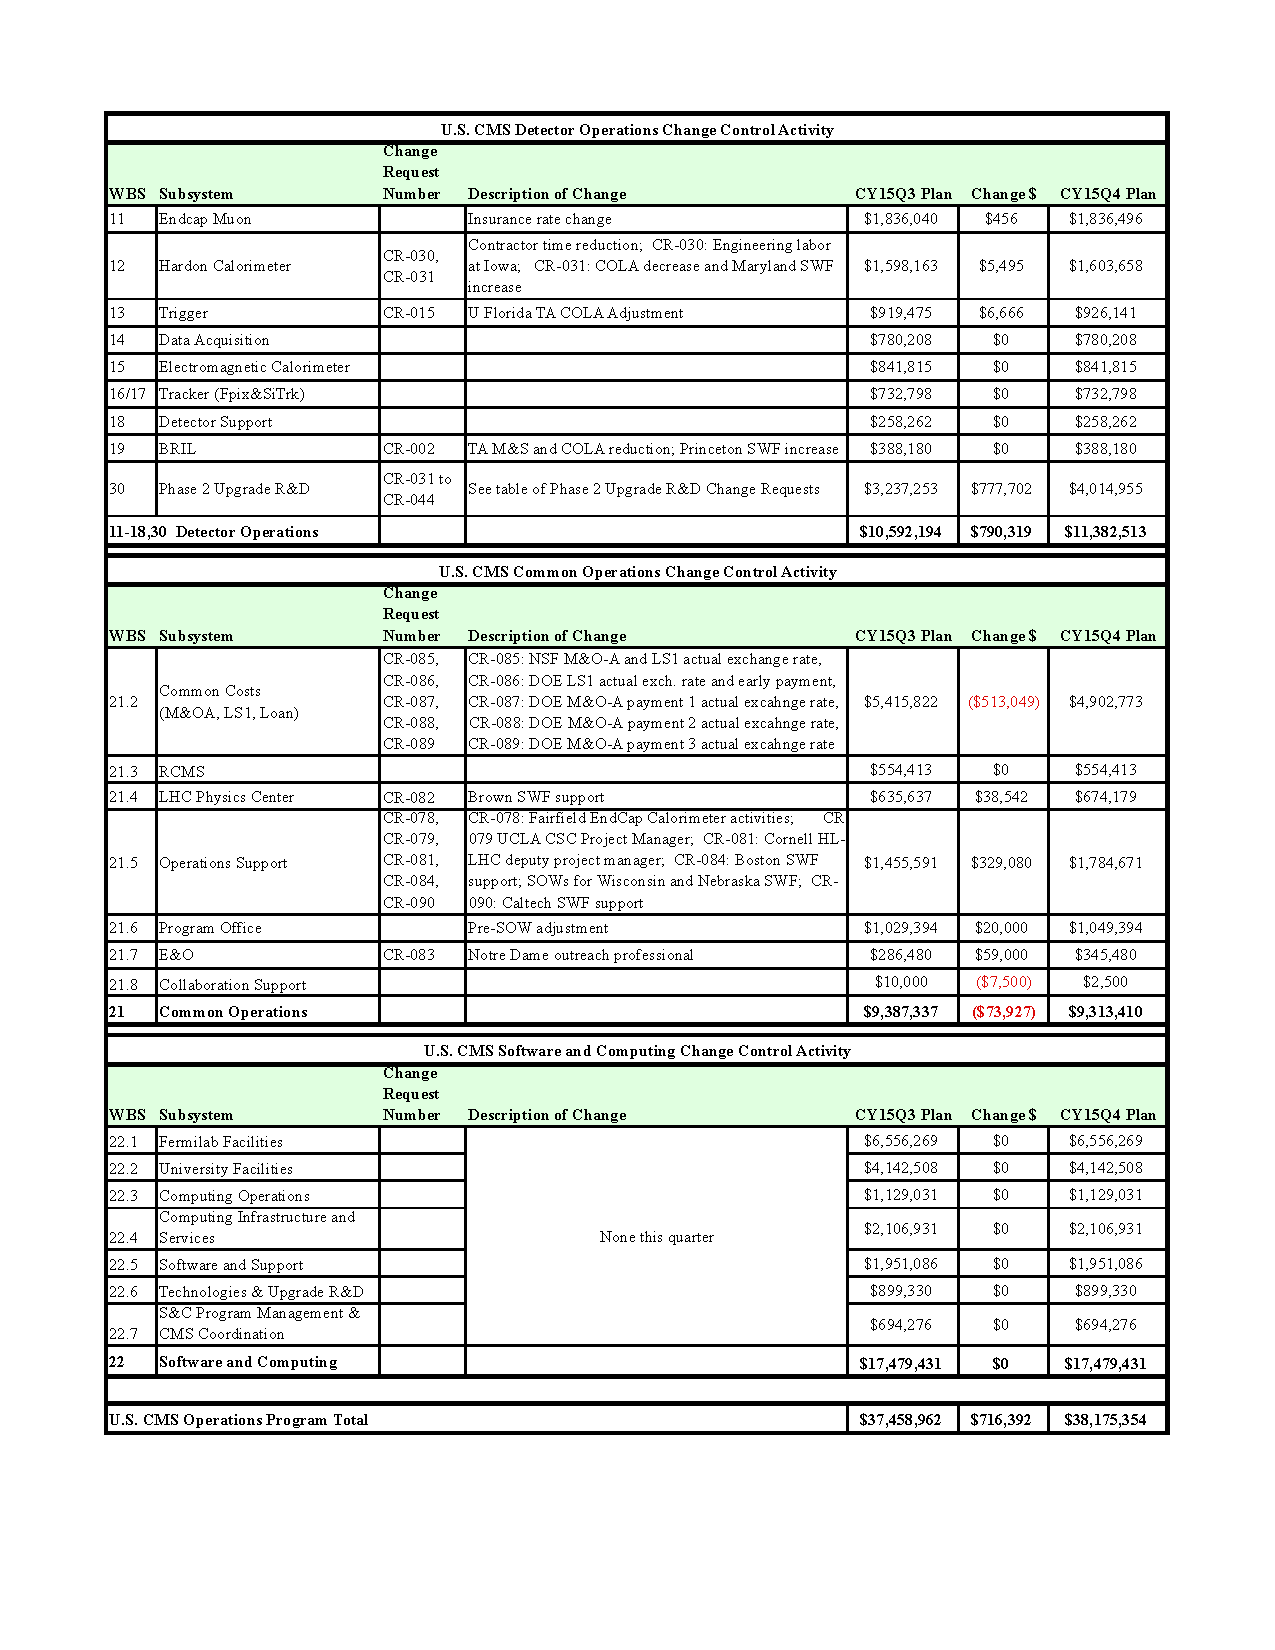
\includegraphics{figures/CY15Q3_Change_Log.pdf}}
    \label{tab:change_log}
  \end{center}
\end{table}

\begin{table}[hbtp]
  \begin{center}
    \caption{Phase 2 (HL-LHC) Upgrade R\&D Change Requests in CY15 Q3}
    \resizebox{4.25in}{!}{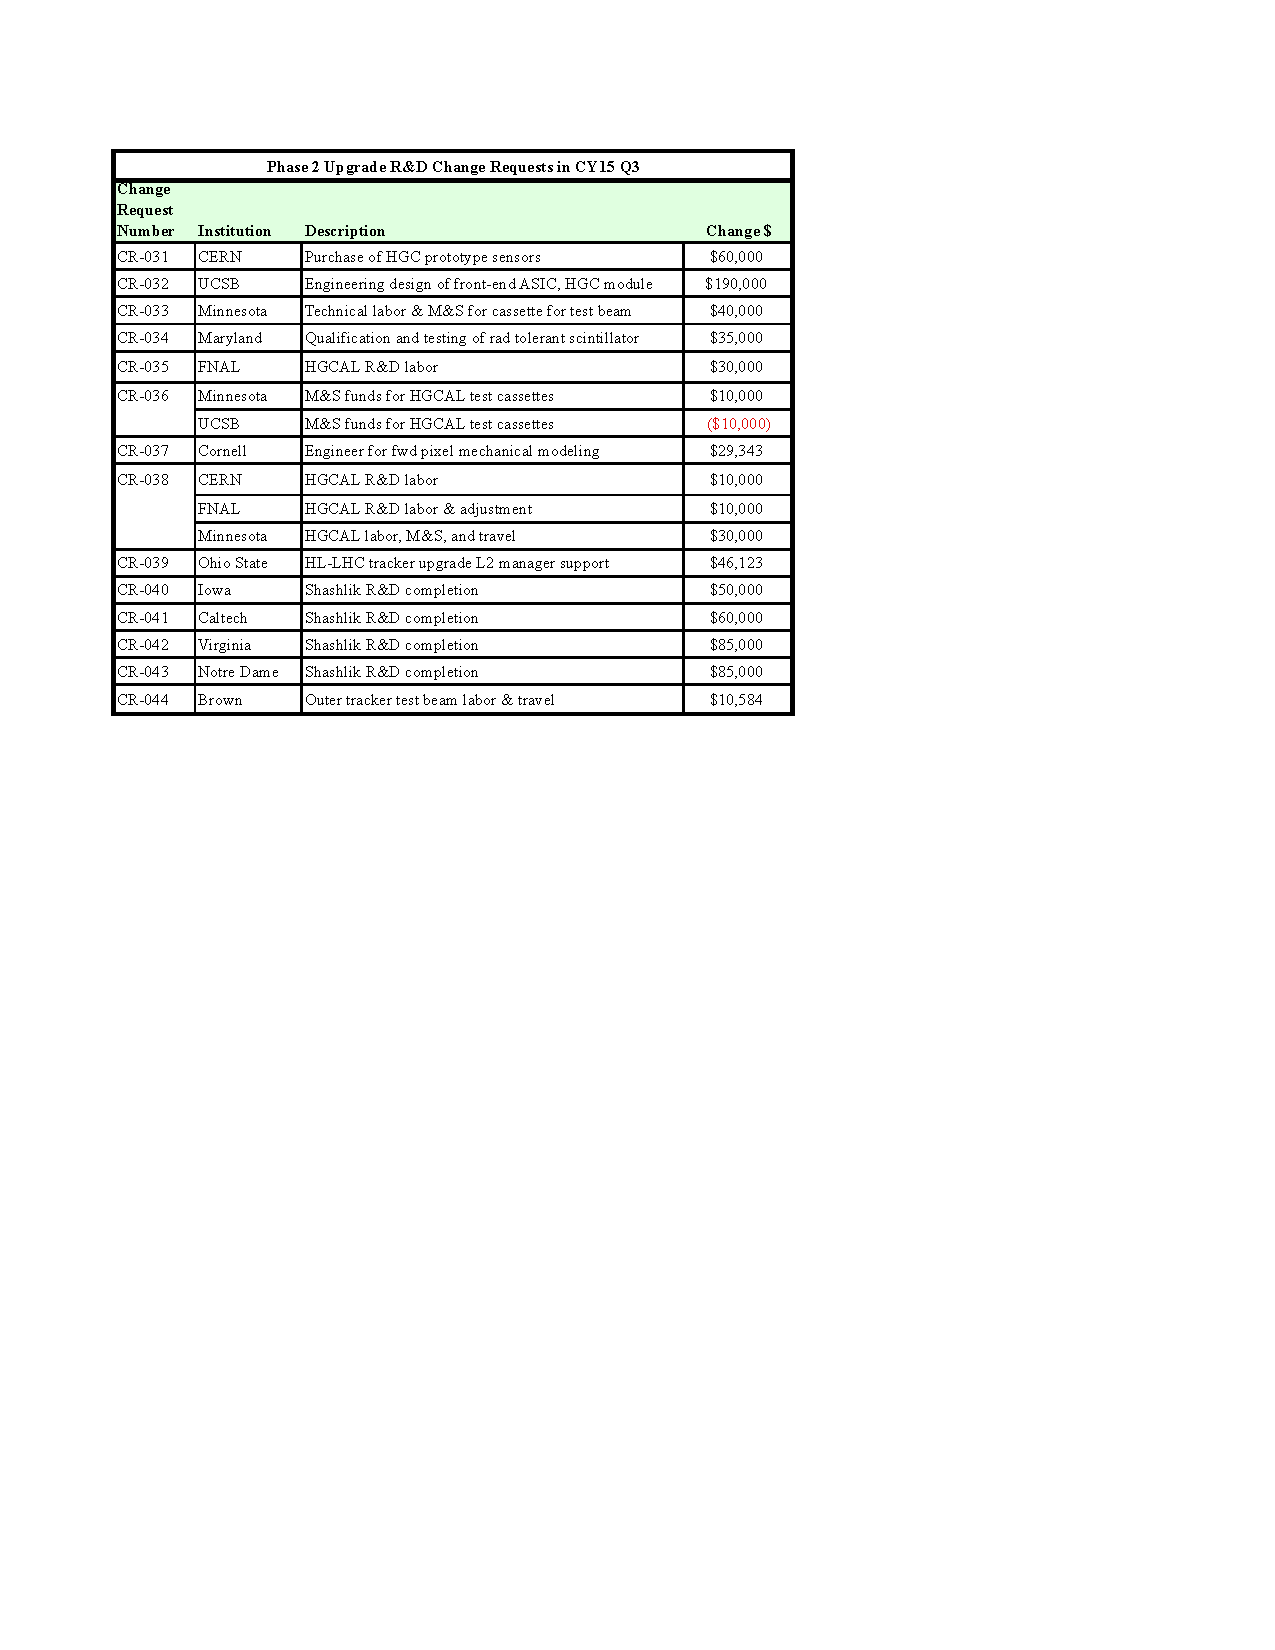
\includegraphics{figures/CY15Q3_Phase2UpgradeChangeLog.pdf}}
    \label{tab:phase2_change_log}
  \end{center}
\end{table}

\begin{table}[hbtp]
  \begin{center}
    \caption{Spending plan at the end of CY15 Q3, for funds from DOE, NSF, and the total.}
    \resizebox{6.25in}{!}{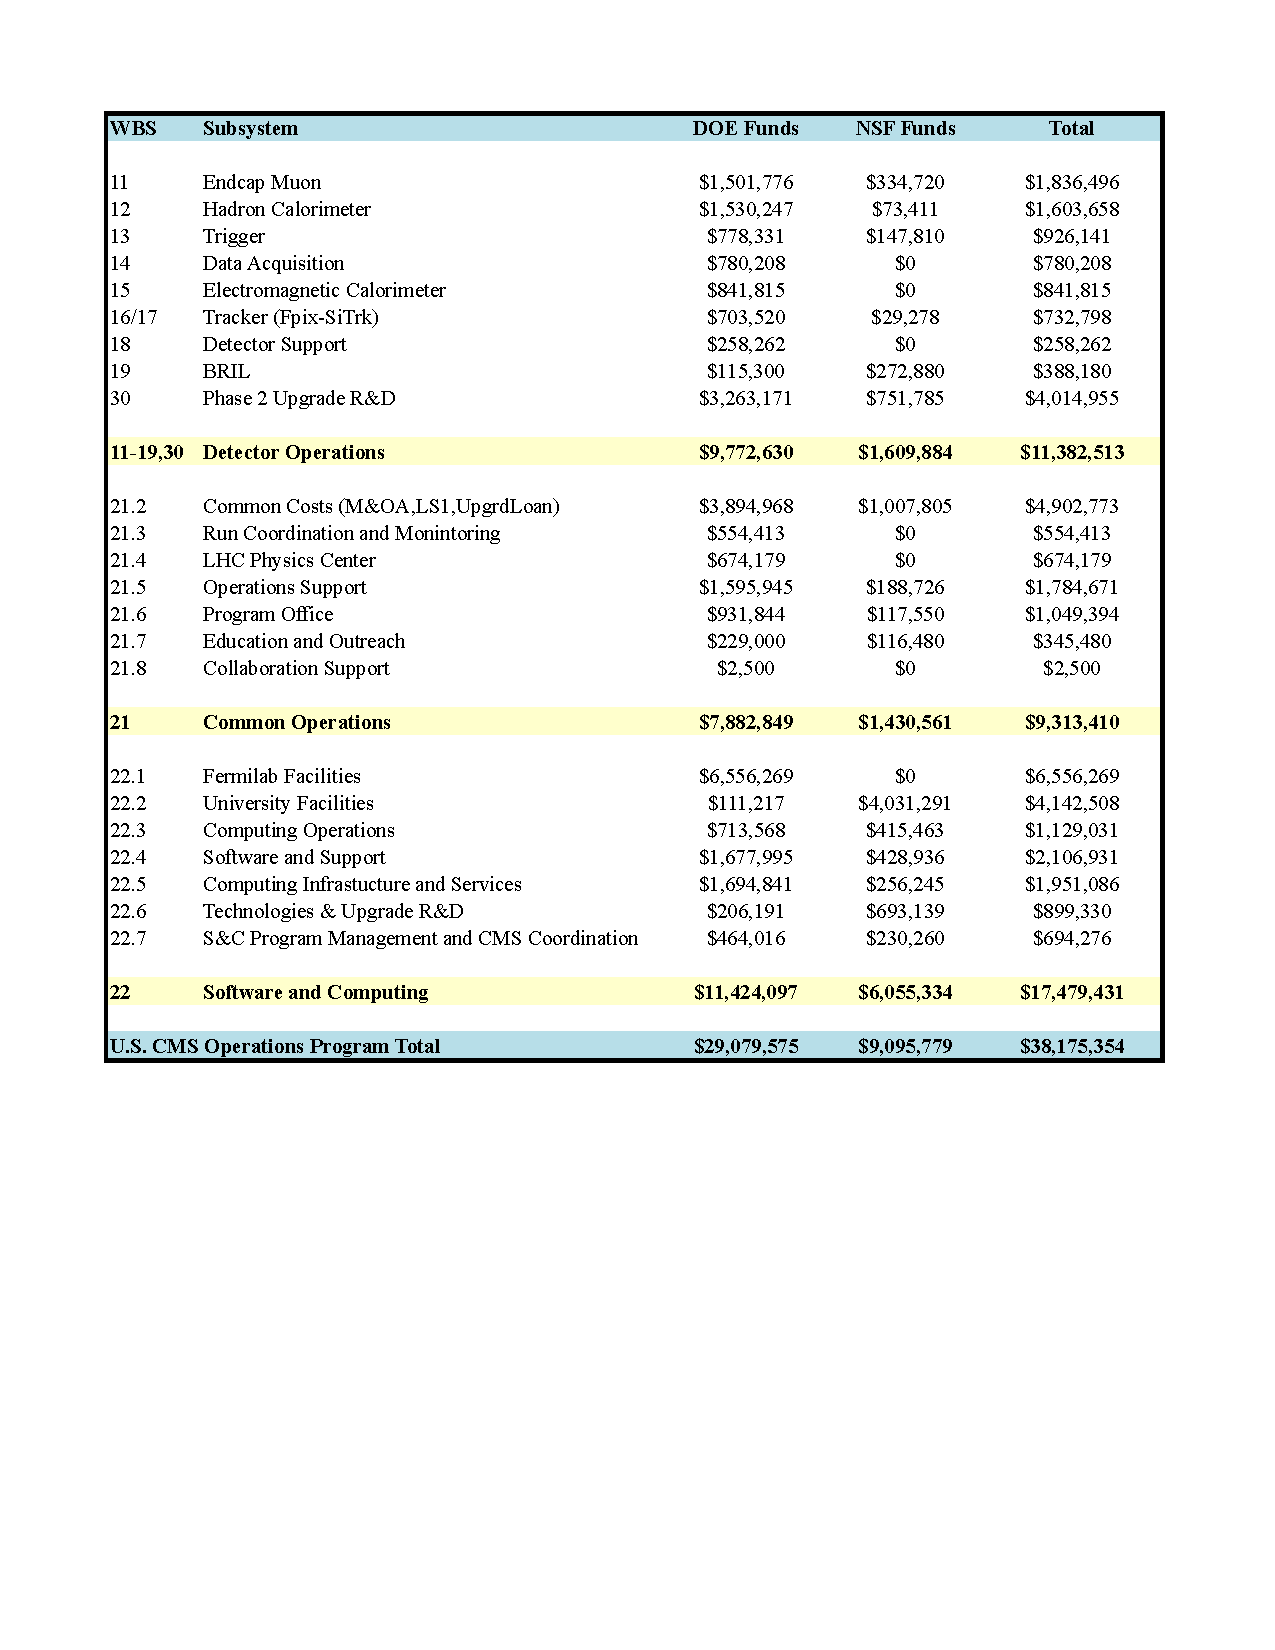
\includegraphics{figures/CY15Q3_Spending_Plan.pdf}}
    \label{tab:spending_plan}
  \end{center}
\end{table}

Once funds have been committed through purchase orders, in the case of DOE, and
sub-awards, in the case of NSF, they are considered obligated.
Figure~\ref{fig:DOE_obligations} shows the obligations in the areas of DetOps,
S\&C, and ComOps, as compared to the spending plan, for DOE funds.  The spending
plan is plotted as if expenditures are carried out in even allocations each month, but this is
intentionally not the case due to equipment purchases and the larger of the transfers to CERN-based
Team Accounts, the latter of which are targeted for when exchange rates are favorable.

Spending through Universities and CERN Team Accounts is budgeted and tracked according
to the calendar year, while spending at Fermilab has historically been budgeted according
to the fiscal year.  Of special note is that this year we have transitioned to
reporting based on calendar year rather than based on fiscal year.  There are two features
of Figure~\ref{fig:DOE_obligations} related to this transition.
First, obligations for DOE spending at Fermilab in the last three months of calendar year 2014
have been included in the plotted obligations for 2015.  Second, to accommodate the three month
offset between fiscal year and calendar year, a buffer of \$3M has been allocated this year,
drawing from carry over from previous years.  This is indicated by the difference between
the solid and dashed blue lines.  Figure~\ref{fig:NSF_obligations} shows the total obligations
and the spending plan, for NSF funds.  Of the \$9M in NSF funding, \$2.5M in subawards went out
this quarter, in addition to spending directly at Princeton.

\begin{figure}[hbtp]
  \begin{center}
    \resizebox{4.5in}{!}{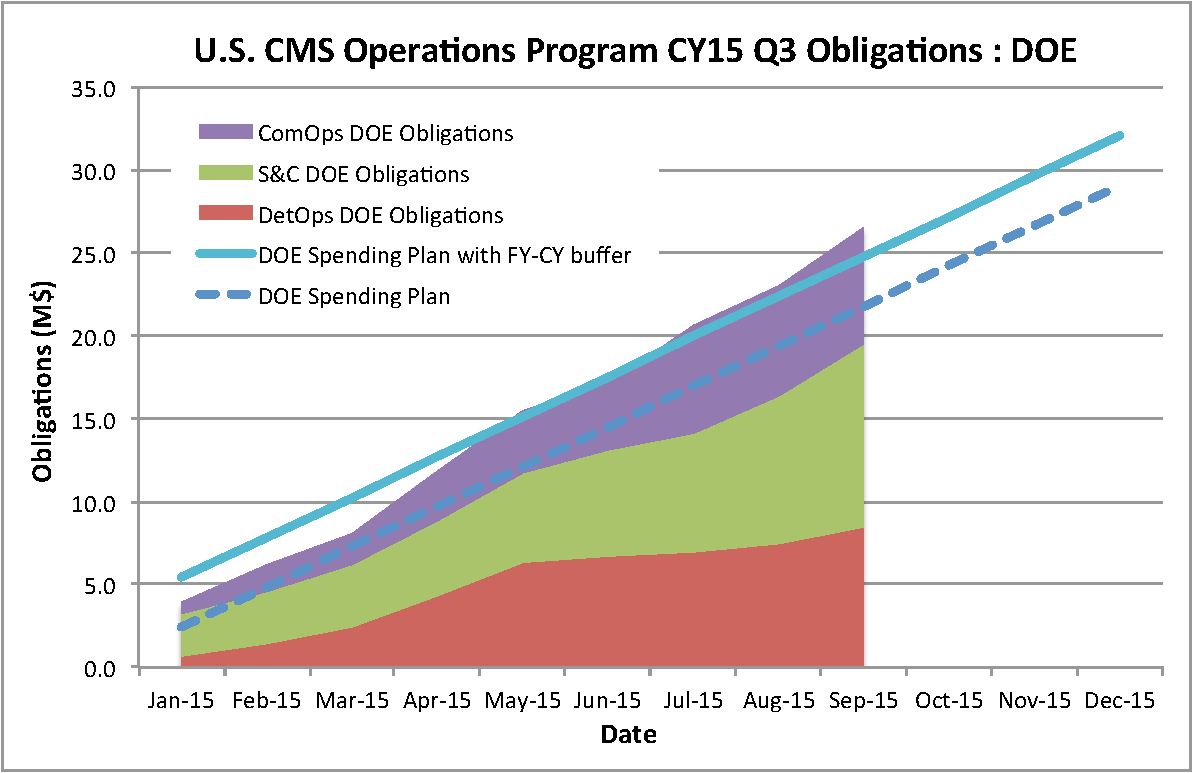
\includegraphics{figures/CY15Q3_DOE_Obligations.pdf}}
    \caption{Obligations and spending plan for DOE funds.  The spending plan
is indicated with the assumption of equal monthly increments just as a rough guide.
The lines show the spending plan with (solid) and without (dashed) a required
buffer to bridge the difference between fiscal year and calendar year for
funds spent at Fermilab, as described in the text.}
    \label{fig:DOE_obligations}
  \end{center}
\end{figure}

\begin{figure}[hbtp]
  \begin{center}
    \resizebox{4.5in}{!}{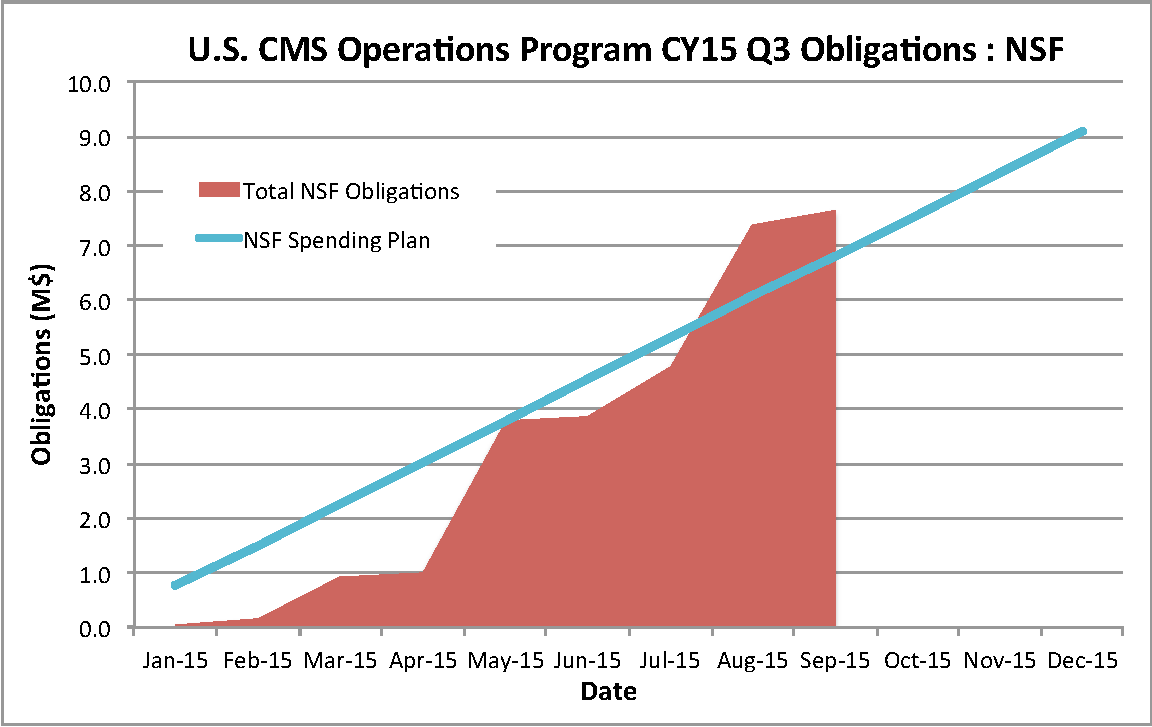
\includegraphics{figures/CY15Q3_NSF_Obligations.pdf}}
    \caption{Obligations and spending plan for NSF funds.  The spending plan
is indicated with the assumption of equal monthly increments as a rough guide.}
    \label{fig:NSF_obligations}
  \end{center}
\end{figure}

Resources deployed at CERN, and paid directly in Swiss francs, account for approximately
28\% of the 2015 spending plan.  This carries considerable exposure to the exchange rate.
A rate of 0.9 CHF/USD has been used for planning, while the actual rate in
CY15 Q3 averaged 0.96 CHF/USD.  Figure~\ref{fig:Team_Accounts} shows the
allocated budgets and year-to-date spending through the Team Accounts that are
used for expenditures at CERN.  Spending for labor and cost of living adjustments
occurs at a fairly constant rate.  Figure~\ref{fig:Team_Accounts} does not include
the last 823K CHF of the Upgrade Common Fund payments and the 3,827K CHF M\&O-A payments,
as these are each made through multiple payments to a separate Team Account.
% Source for exchange rate average:
% http://www.oanda.com/currency/historical-rates/

\begin{figure}[hbtp]
  \begin{center}
    \resizebox{4.5in}{!}{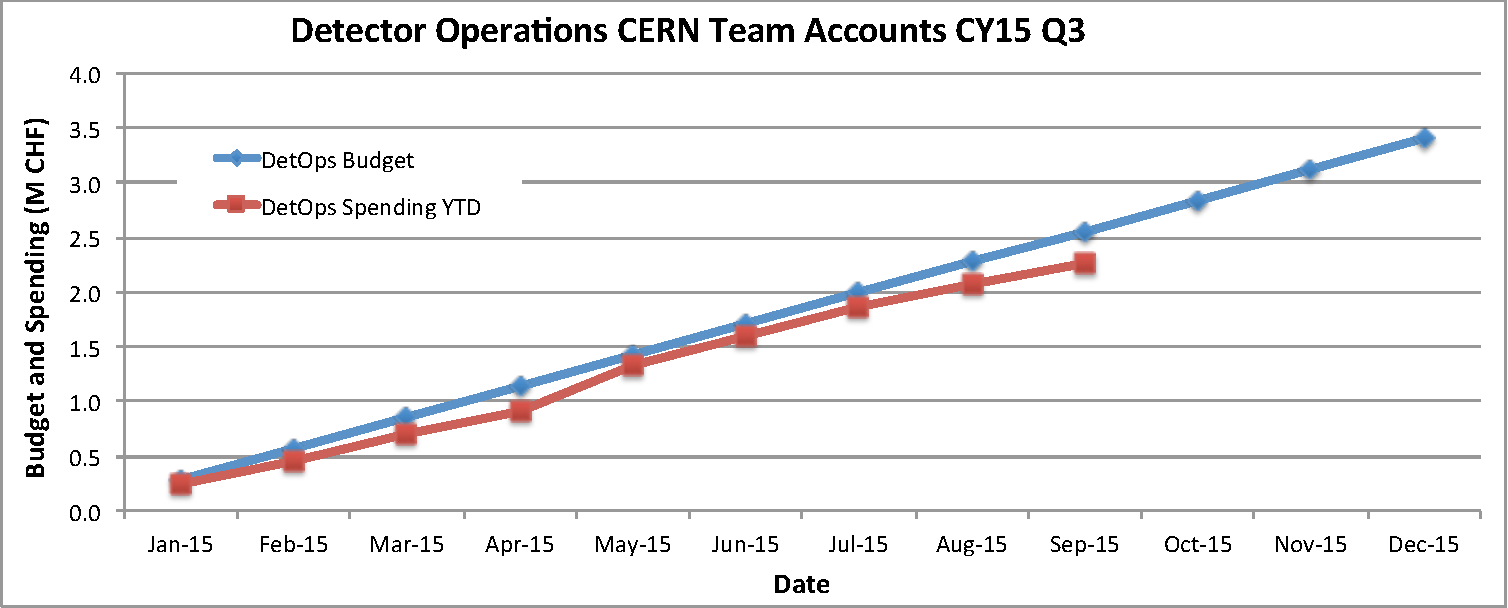
\includegraphics{figures/CY15Q3_TA_DetOps.pdf}}
    \resizebox{4.5in}{!}{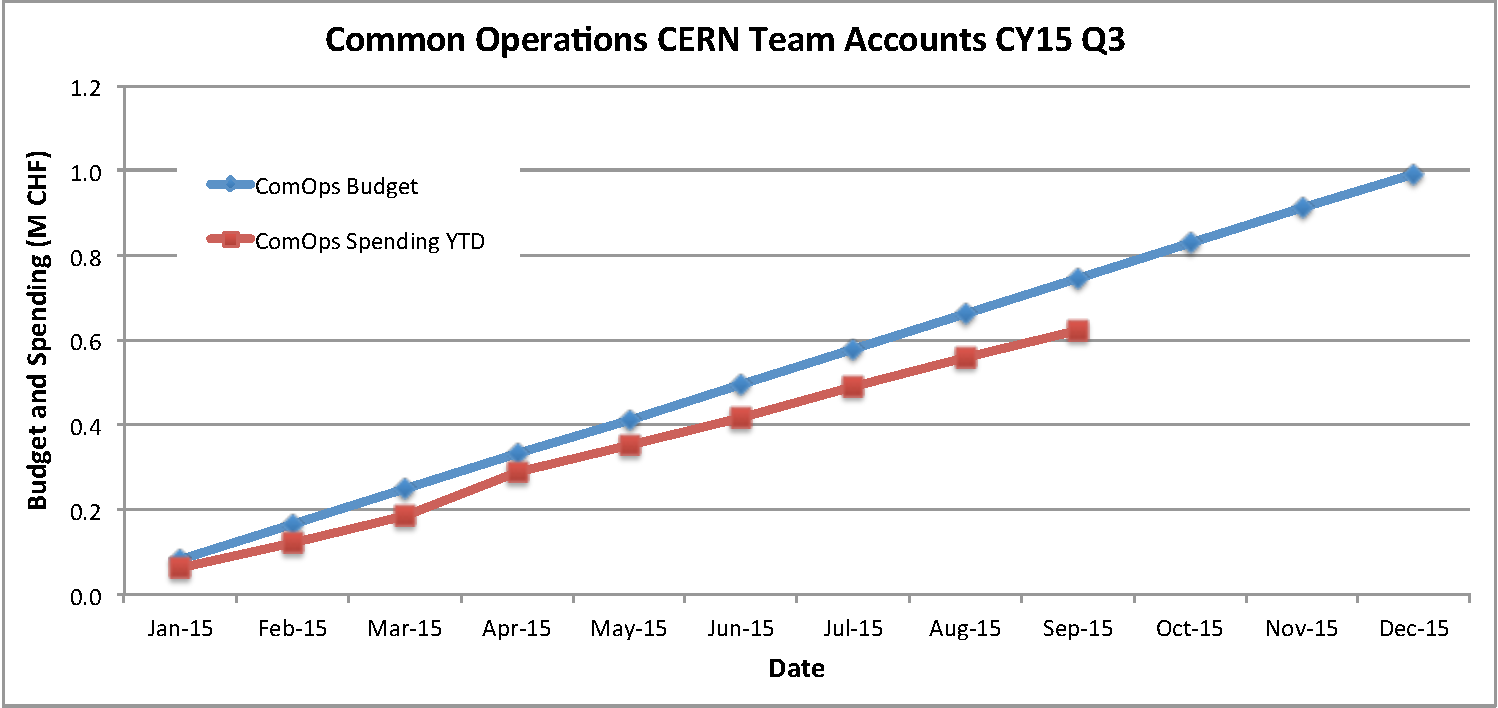
\includegraphics{figures/CY15Q3_TA_ComOps.pdf}}
    \resizebox{4.5in}{!}{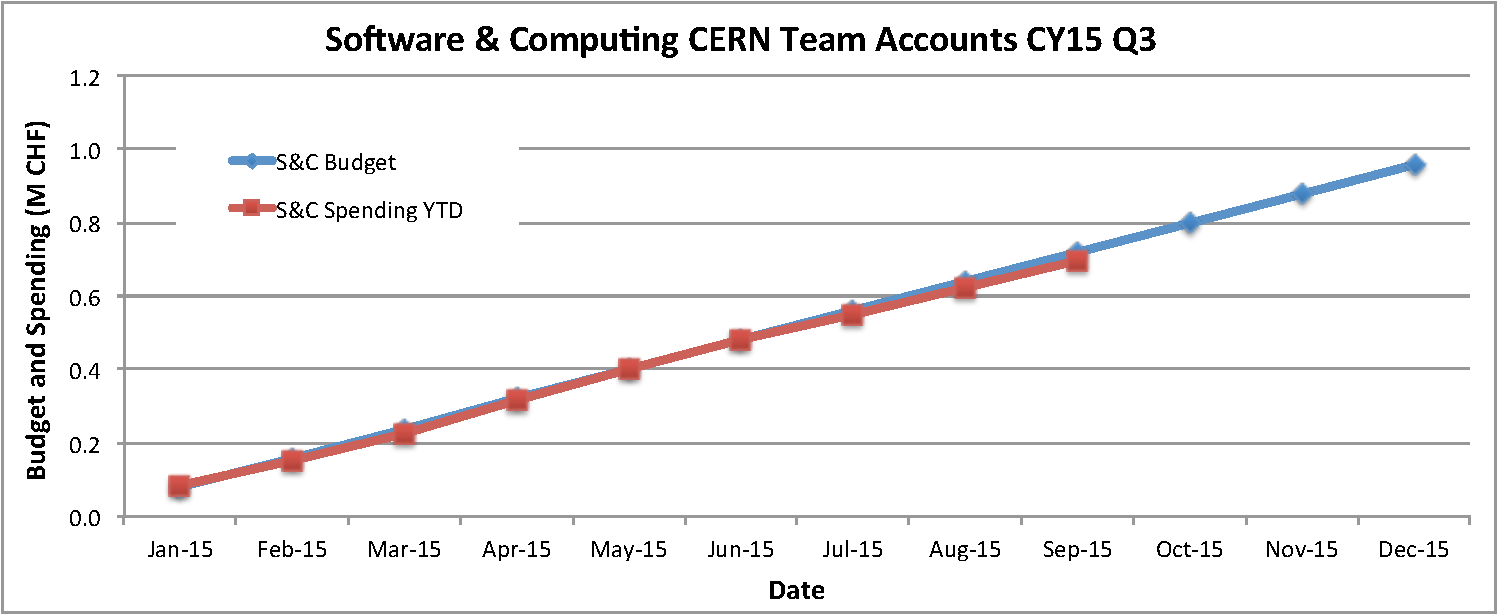
\includegraphics{figures/CY15Q3_TA_S&C.pdf}}
    \caption{Budget plan and year-to-date spending, in Swiss francs, through DetOps (top), ComOps (middle),
and S\&C (bottom) Team Accounts.}
    \label{fig:Team_Accounts}
  \end{center}
\end{figure}

